\documentclass[11pt,a4paper]{article}
\usepackage{ctex}
\usepackage[utf8]{inputenc}
\usepackage{geometry}
\usepackage{fancyhdr}
\usepackage{enumitem}
\usepackage{titlesec}
\usepackage{amsmath} % Added for math equation support
\usepackage{graphicx} % Added for including graphics
\usepackage{titling}
\usepackage{subcaption}

\usepackage{multicol}
\usepackage{listings}
\usepackage{booktabs}
\usepackage{multirow}

\usepackage[hidelinks]{hyperref}
% \usepackage[style=authoryear]{biblatex} % Use biber backend
% \addbibresource{../../paper.bib} % Specify the .bib file
% Define \lll
\newcommand{\lll}{\mathrel{<\!\!<\!\!<}}
% Define \ggg
\newcommand{\ggg}{\mathrel{>\!\!>\!\!>}}
\geometry{margin=0.5in}
\titleformat{\section}{\large\bfseries}{\thesection}{0.5em}{}

% title context and style setting
\title{周报-向嘉豪(2024-11-18)}
\setlength{\droptitle}{-6em} % Reduce space begin the title
% Redefine \maketitle to display only the title
\renewcommand{\maketitle}{
  \begin{center}
    \LARGE\bfseries\thetitle
  \end{center}
}

\begin{document}

\maketitle


% Custom Abstract
\noindent \textbf{Abstract}: 本周主要对OPO(Optimization of Permutation Operation)算法进行了优化和重构。通过引入贪心递归策略解决了局部最优解问题,并重构了PPO类结构以提高代码可维护性。将优化后的OPO算法应用于AES的ShiftRow操作,在STM32L475平台上进行测试,相比\cite{Schwabe2016}的实现,执行周期数从8932降至8068,性能提升9.7\%,同时降低了Flash内存占用。

\noindent \textbf{下周计划}: 完成论文撰写并将重。

\subsection{OPO算法优化}
此前实现的Optimization of Permutation Operation (OPO) 图~\ref{fig:old_opo},存在求解,遇见局部最优解的问题,通过引入贪心递归策略,来找到全局最优解,优化后的OPO算法如图~\ref{fig:new_opo}所示。

\begin{figure}[h]
  \centering
  \begin{subfigure}[b]{0.48\textwidth}
    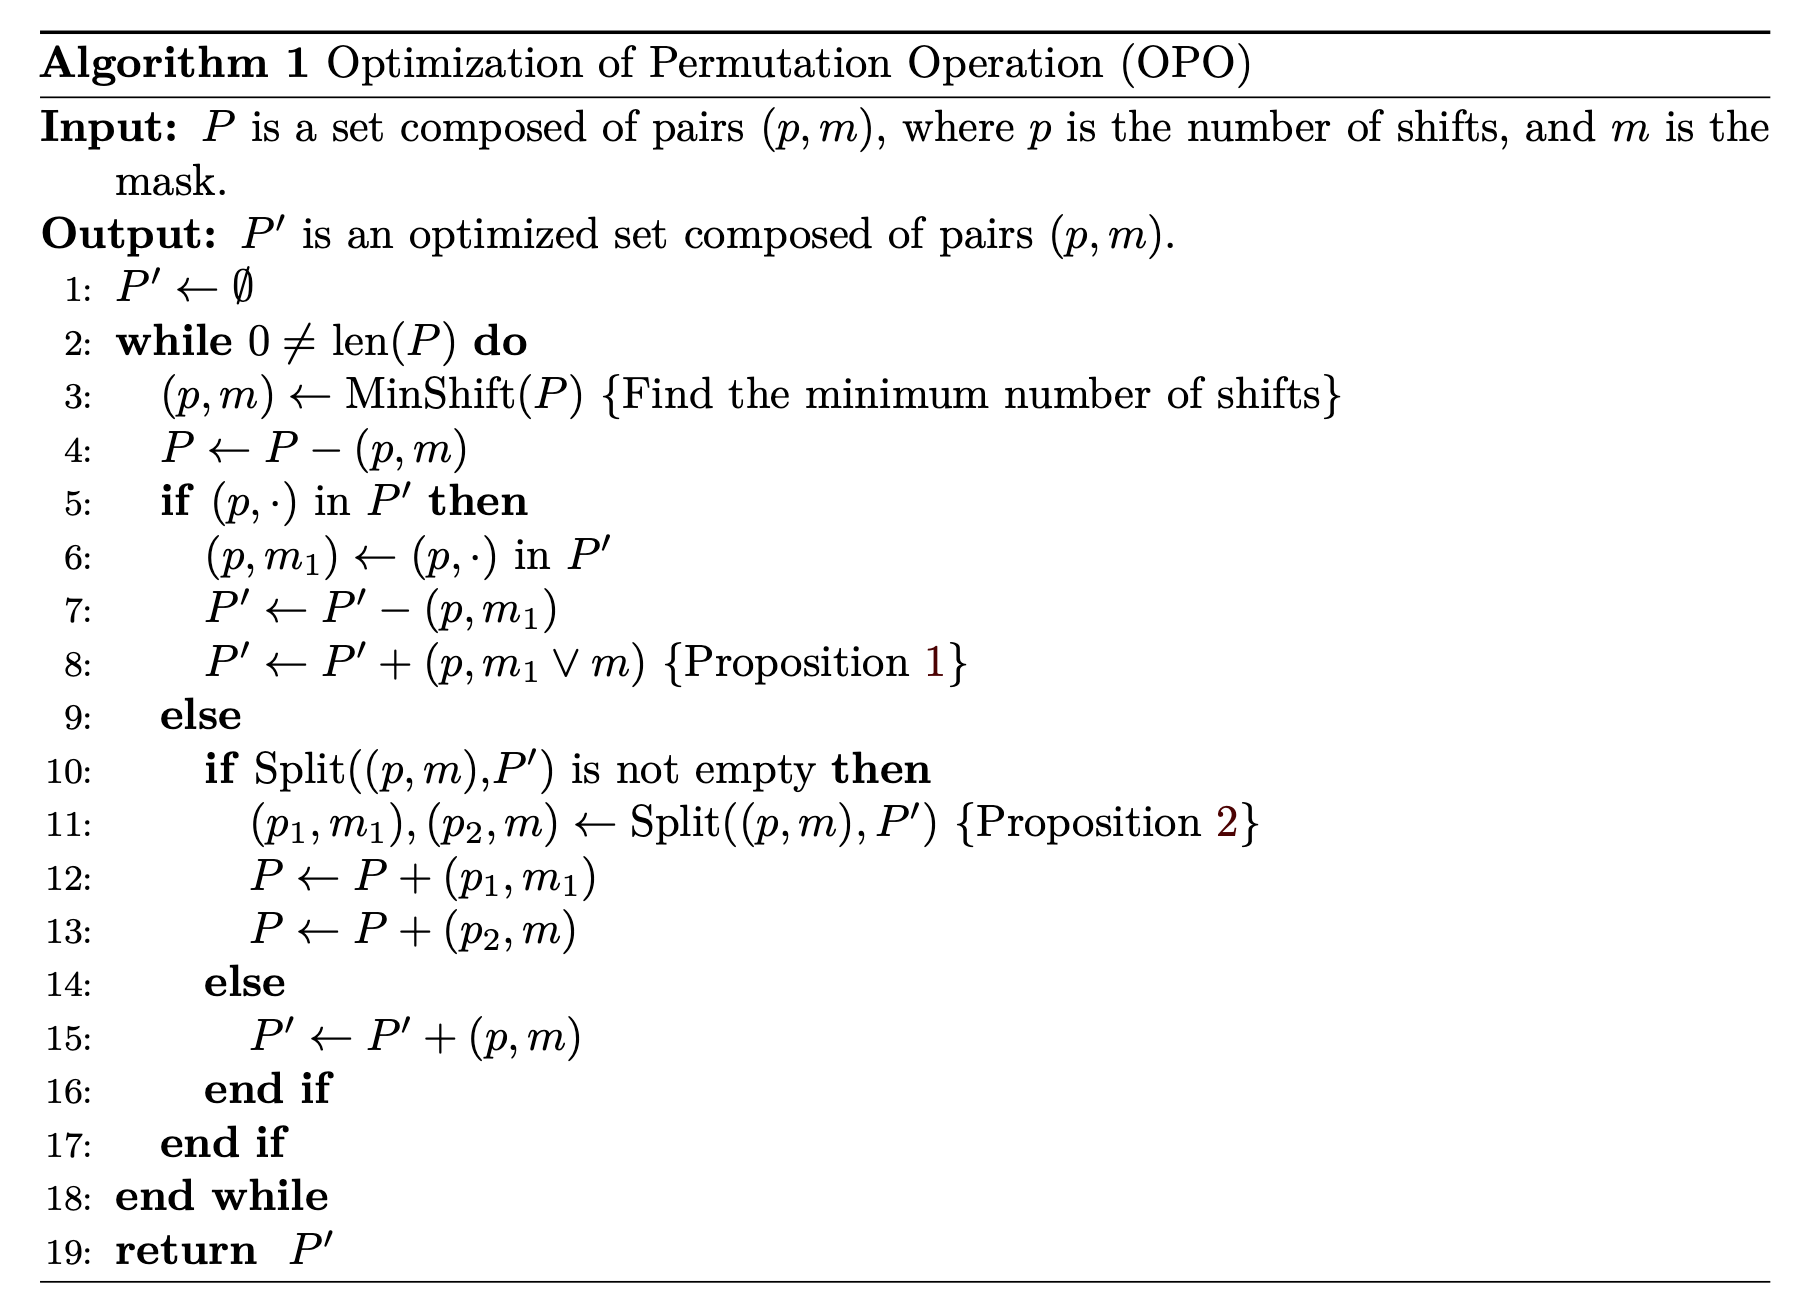
\includegraphics[width=0.7\textwidth]{./fig/old_opo.png}
    \caption{原始OPO算法}
    \label{fig:old_opo}
  \end{subfigure}
  \begin{subfigure}[b]{0.48\textwidth}
    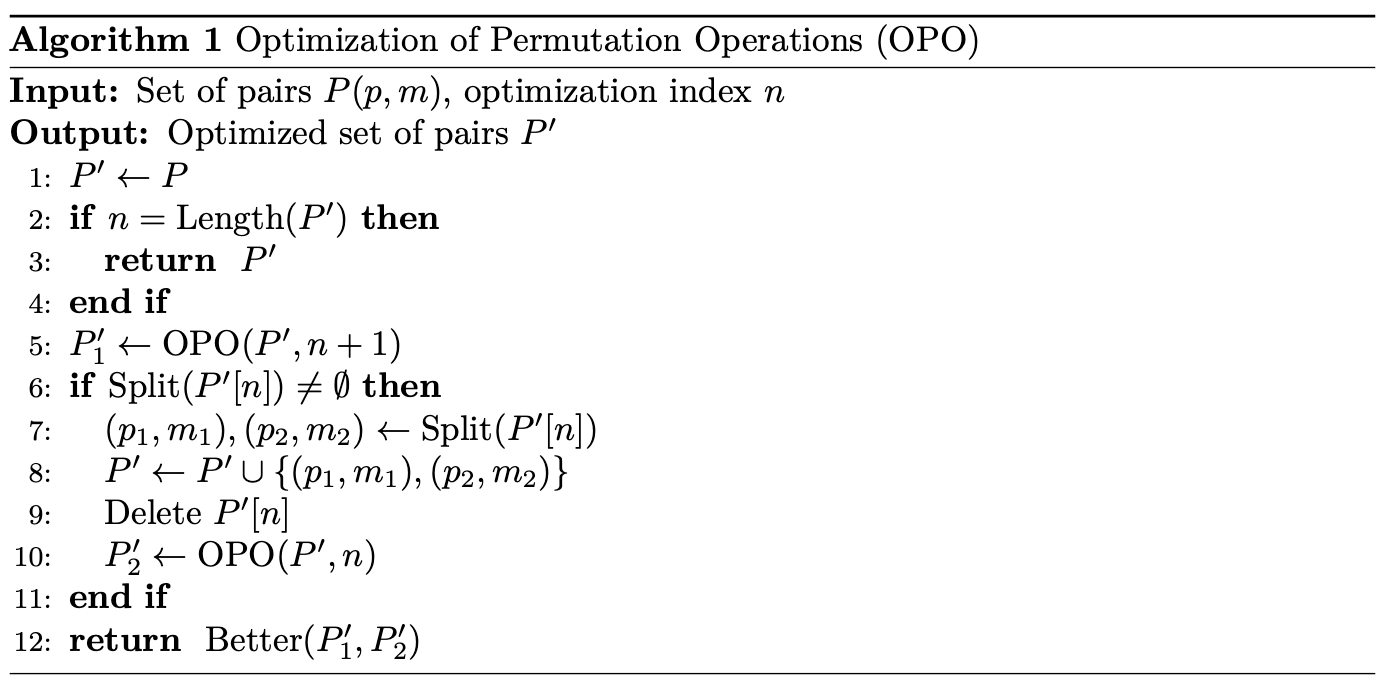
\includegraphics[width=\textwidth]{./fig/new_opo.png}
    \caption{优化后OPO算法}
    \label{fig:new_opo}
  \end{subfigure}
  \caption{OPO算法优化}
\end{figure}

在对图~\ref{fig:new_opo}实现时,发现旧版存在,需要手动计算中间寄存器与汇编转化的问题,因此我们重构了,使用PPO类来结构化组织PPO操作,如图~\ref{fig:ppo}所示。 从之前的 [(3, [8, 11, 10, 2]), (4, [5, 10, 4, 6, 12, 15]), (5, [14, 9])]表示的操作序列,转化为PPO类的操作序列,[('and', 'r1', 'r0', '0xaa000000'), ('ror', 'r1', 'r1', 0), ('or', 'r14', 'r14', 'r1')], 类汇编组织结构。

\begin{figure}[h]
  \centering
  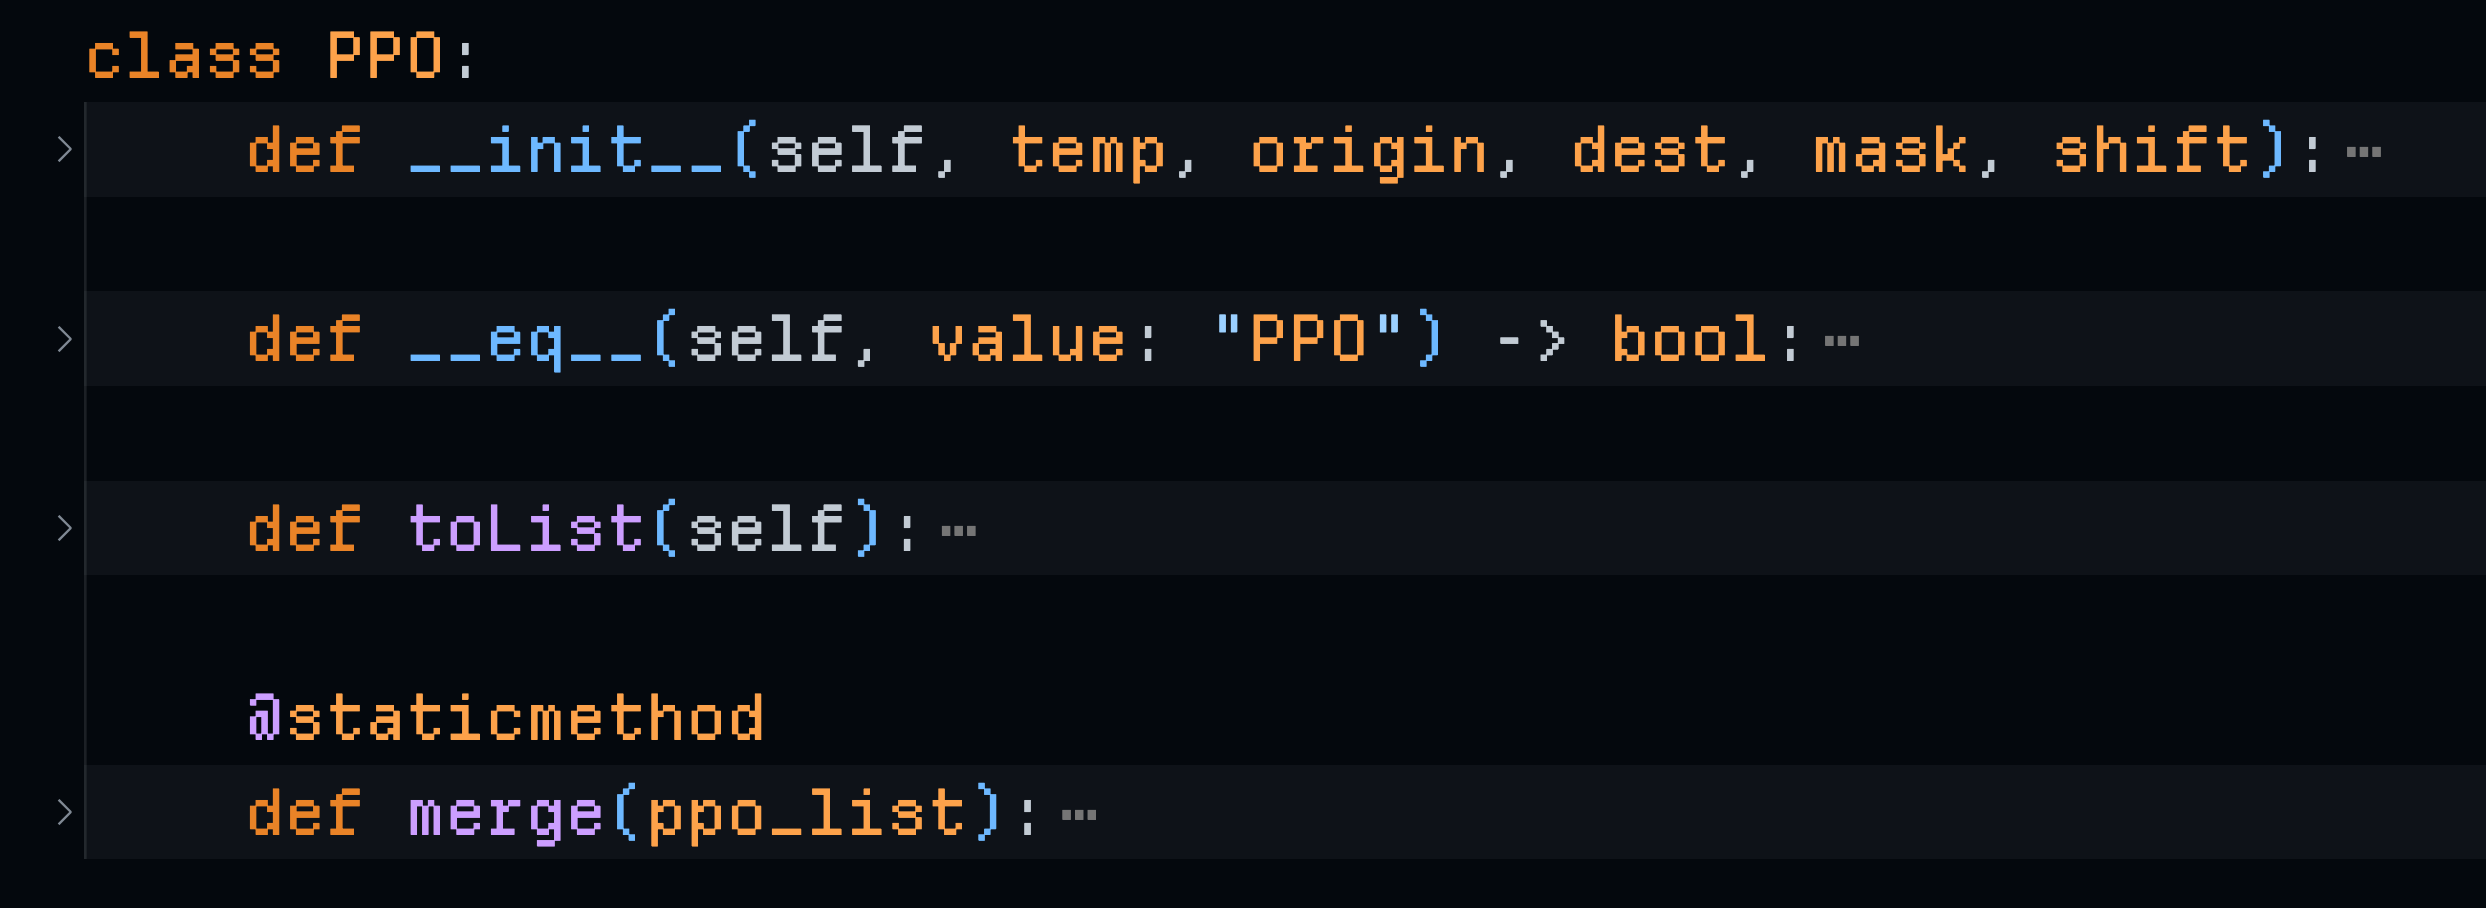
\includegraphics[width=0.5\textwidth]{./fig/ppo_class.png}
  \caption{PPO类结构}
  \label{fig:ppo}
\end{figure}

\subsection{OPO优化AES算法}
在\cite{Schwabe2016}中提出的AES算法的基础上,我们使用OPO算法进行优化,通过OPO算法优化后的AES算法的ShiftRow。以下为其中未优化代码Listing~\ref{lst:shift_row}和优化后代码Listing~\ref{lst:opt_shift_row}的对比。通过我们的优化,可以看出其中的PPO操作序列减少了2次。

% Replace verbatim blocks with:
\begin{figure}[ht]
  \begin{minipage}{\textwidth}
  \begin{multicols}{2}
  \begin{lstlisting}[
      caption={原始汇编代码实现},
      label={lst:shift_row},
      basicstyle=\ttfamily\small,
      numbers=left,
      frame=single]
# 操作序列
r1 r0 r14 0xaa000000 0
r1 r0 r14 0x2a 2
r1 r0 r14 0xa00 4
r1 r0 r14 0x20000 6
r1 r0 r14 0x80 26
r1 r0 r14 0xa000 28
r1 r0 r14 0xa80000 30
# 汇编代码
uxtb.w r12, r9
ubfx r5, r9, #14, #2
eor r12, r12, r5, lsl #8
ubfx r5, r9, #8, #6
eor r12, r12, r5, lsl #10
ubfx r5, r9, #20, #4
eor r12, r12, r5, lsl #16
ubfx r5, r9, #16, #4
eor r12, r12, r5, lsl #20
ubfx r5, r9, #26, #6
eor r12, r12, r5, lsl #24
ubfx r5, r9, #24, #2
eor r12, r12, r5, lsl #30
  \end{lstlisting}
  \columnbreak
  \begin{lstlisting}[
      caption={优化后汇编代码实现},
      label={lst:opt_shift_row},
      basicstyle=\ttfamily\small,
      numbers=left,
      frame=single]
# 操作序列
r1 r0 r14 0xaa000000 0
r1 r0 d0 0x2a02a 2
r1|d0 r0 r14 0x8a00 4
r1|d0 r0 r14 0x2880 26
r1 r0 r14 0xa80000 30
# 汇编代码
uxtb.w r12, r9
and r5, r9, #0x2a02a
eor r12, r12, r5, ror #2
and r5, r9, #0x8a00
eor r12, r12, r5, ror #6
and r5, r9, #0x2880
eor r12, r12, r5, ror #26
and r5, r9, #0xa80000
eor r12, r12, r5, ror #30
  \end{lstlisting}
  \end{multicols}
  \caption{汇编代码实现对比分析}
  \label{fig:code_comparison}
  \end{minipage}
\end{figure}

由于性能测试框架和测试芯片的不同,\cite{Schwabe2016}中给出的实现周期数为3234,而我们将其代码放入我们LCB测试框架stm32l475测试出来的数据为8932。为公平比较,此处我们将使用LCB,测试我们的优化代码,从表~\ref{tab:shift_row}中可以看出,我们的优化代码的周期数为8068,提升了9.7\%。

\begin{table}[ht]
    \centering
    \caption{AES算法实现性能对比}
    \label{tab:shift_row}
    \begin{tabular}{lccc}
        \toprule
        实现方案 & 优化等级 & 周期数 & Flash大小(字节) \\
        \midrule
        \multirow{1}{*}{\cite{Schwabe2016}} 
            & O3 & 8,932 & 27,100 \\
        \midrule
        \multirow{1}{*}{本文工作} 
            & O3 & \textbf{8,068} & \textbf{25,948} \\

        \bottomrule
    \end{tabular}
\end{table}

\newpage
% Add some vertical space to push content to bottom if needed
\vfill


% Include the bibliography
\bibliographystyle{alpha}
\bibliography{../../paper}

\end{document}